%% Function Generator


\documentclass[12pt,a4paper]{article}


\newcommand{\docconfig}{../../../Latex_set_up}
\newcommand{\imagefolder}{../figure}



\usepackage{float}
\usepackage{polyglossia}
\usepackage{graphicx,wrapfig,lipsum}
\usepackage{xspace}
\usepackage{glossaries}
\usepackage{color}
\usepackage{fontspec}

\usepackage{blindtext}
\usepackage[utf8]{inputenc}
\usepackage{fancyhdr}

\usepackage{booktabs} %for Excel
\usepackage{multirow}
\usepackage{pbox}

\usepackage{hyperref}

\usepackage{siunitx}
\usepackage{comment}
\usepackage{enumitem}
\usepackage{amsmath}

\usepackage{tabularx} % for table adjustment
%
\usepackage[a4paper ,total={6in, 8in}]{geometry}
%\usepackage[showframe=true]{geometry}
% XeLaTeX!
% ============================================================ %
% HEBREW support via polyglossia %
% ============================================================ %
%\usepackage{polyglossia}
\defaultfontfeatures{Mapping=tex-text, Scale=MatchLowercase}
\setdefaultlanguage{english}
\setotherlanguage{hebrew}
\newfontfamily\hebrewfont[Script=Hebrew]{David}
% Use \begin{hebrew} block of text \end{hebrew} for paragraphs.
% Use \texthebrew{ } and \textenglish{ } for short texts.
% ============================================================ %
\newcommand{\te}[1]{\textenglish{#1}}


\newcommand{\thh}[1]{\texthebrew{#1}}
%Hyper Link Setup
\hypersetup{
	colorlinks=true,
	linkcolor=blue,
	filecolor=magenta,      
	urlcolor=blue,
}

%% DMM and link to wiki
\newcommand{\dmm}{\href{https://en.wikipedia.org/wiki/Multimeter}{\te{(DMM)}}}

\begin{document}
	\begin{hebrew}
		\title{מחולל אותות}
		\maketitle
	\end{hebrew}
\pagebreak
\begin{hebrew}
	\section{רקע כללי}
	מחולל אותות (באנגלית: \te{Function Generator}) הוא מכשיר אלקטרוני המייצר אותות מתח חילופין הדומים לאלה המופיעים במעגלים חשמליים.
	המחולל מסוגל לספק מתחי חילופין בעלי צורות גל שונות ,למשל גל סינוסי,גל שונות,למשל גל סינוסי,גל ריבועי וגל משולש ,בתדר רצוי ובמשרעת (אמפליטודה) הניתנת לשינוי,כמו כן אפשר להוסיף מתח ישיר(חיובי או שלילי) למתח חילופין. \\
	האות היוצא מהמחולל מכיל תמיד עיוותים למיניהם יחסית לצורת גל התאורטית ,בדרך כלל גודלם אחוז עד עשירית אחוז מהגל המקורי .
	סטייה זו מוגדרת בשם 
	\te{THD - total harmonic distortion} . \\
	
	\section{\thh{סוגי המכשירים במעבדה}}
	\begin{enumerate}
		\item 
		\te{GFG - 8219A}
			\begin{figure}[h]
				\centering
				\includegraphics[scale=0.3]{"\imagefolder/GFG-8219A/GFG-8219A"}
			%	\caption{}
				\label{fig:gfg-8219a}
			\end{figure}
		\item 
		\te{Agilent - 33220A}
			\begin{figure}
				\centering
				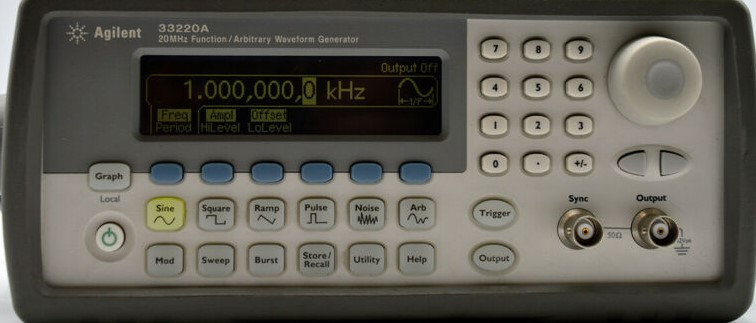
\includegraphics[width=0.6\linewidth]{../figure/33220A/product}
				\caption{}
				\label{fig:product}
			\end{figure}
	\end{enumerate}
\end{hebrew}

\pagebreak

\begin{hebrew}
	\section{פירוט על כל דגם}
	\subsection{GFG-8219A}


	\begin{figure}[!htb]
	\begin{minipage}{0.48\textwidth}
		\centering
		
\includegraphics[width=.7\linewidth]{../figure/GFG-8219A/main}
		
	\end{minipage}
	\hfill
	\begin{minipage}{0.48\textwidth}
		\centering
		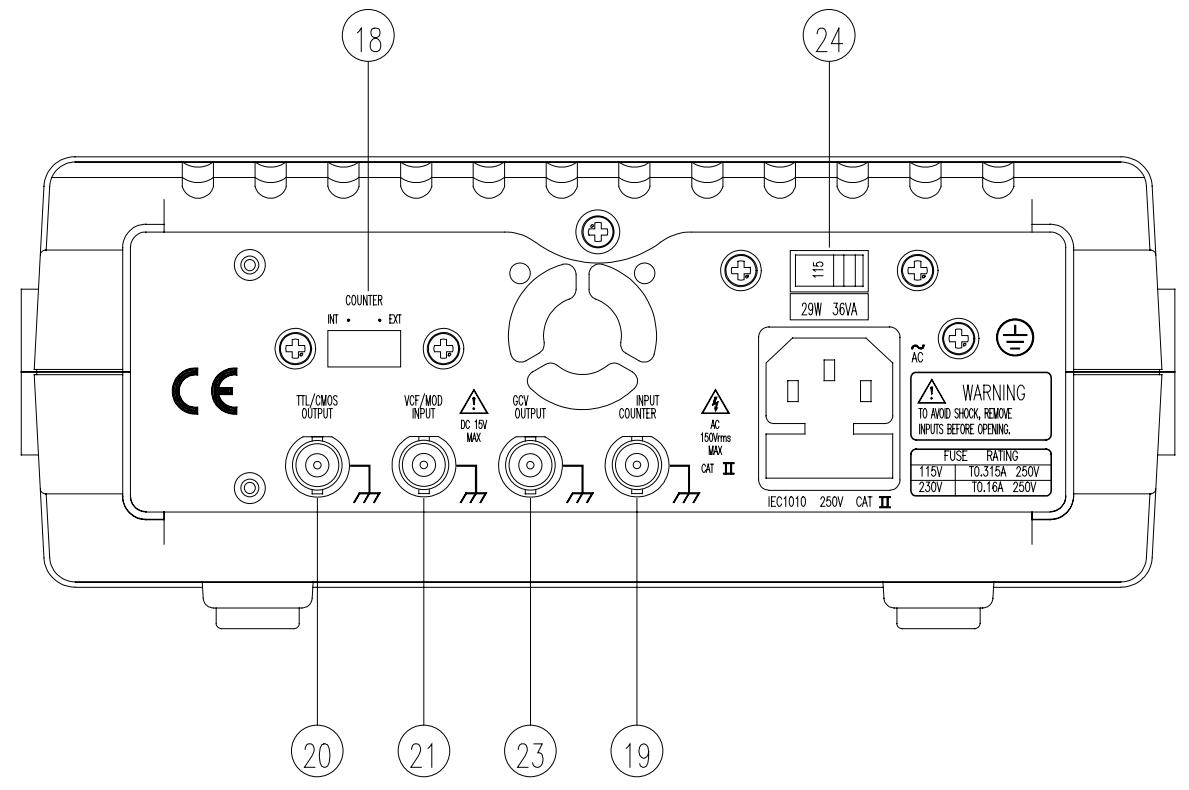
\includegraphics[width=.7\linewidth]{../figure/GFG-8219A/behind main}
		\begin{hebrew}
		\end{hebrew}
	\end{minipage}
\end{figure}

	
	\begin{enumerate}
		\item
		כפתור הפעלה
		\item
		זמן שער
		\item
		במצב מונה חיצוני, המחוון הוא
		מואר כאשר תדר המוצא גדול מ-
		הטווח שנבחר.
		\item
		מראה את התדר החיצוני
		\item
		מראה את גודל התדר באות (כמו $ K =10 ^3 $)
		\item
		מציין את זמן השער הנוכחי.
		\item
		בחירת טווח התדרים הנדרש על ידי לחיצה על
		כפתור לחיצה רלוונטי בלוח.
		\item
	לבחירת צורת הגל(מרובע,משולש,סינוסי)
		\item
		משוך החוצה וסובב את הבורר כדי להתאים את מחזור החובה של
		צורת הגל.
		\addtocounter{enumi}{1}
		\item
		משוך את הבורר כדי לבחור רמת \te{DC} כלשהי
		בין $ \pm \SI{10}{\volt}$ ,סובב עם כיוון השעון כדי להגדיר
		צורת גל ברמת \te{DC} חיובית ולהפוך לשלילה
		צורת גל ברמת \te{DC}.
		\item
		כדי לעלות או להוריד את האמפליטודה סובב עם כיוון השעון ל- \te{MAX}.
			\\
			\textbf{\te{12a}.}
		לחץ על הכפתור כדי לבצע הנחתה ב $ -\SI{20}{\decibel} $
		\item
		לחץ וסובב עם כיוון השעון את הבורר לתדר מקסימום
		והפוך לתדר מינימום.

		משוך את הכפתור כדי להתחיל את פעולת  \te{sweep}    האוטומטית
		מגבלת התדרים העליונה נקבעת על ידי הכפתור
		עמדה.
		\item
		בורר הנועד לקבוע  זמן ה\te{sweep}
		ממהיר לאיטי.
		וכדי לעבוד בצורה לוגריתמית אז יש למשוך את הבורר.
		\addtocounter{enumi}{8}
		\item
		
		זו יצאה המוציאה ערך 
		\te{DC}
		המשתנה בתלות תדר.
		
		
	\end{enumerate}

				\begin{hebrew}
		לפירוט נוסף אפשר לפנות ל:
		\href{https://datasheet.octopart.com/GDM-8245-Instek-datasheet-11997973.pdf}{\te{User Manual}}
	\end{hebrew}
	\pagebreak
	\subsection{Agilnet 33220A}

% TODO: \usepackage{graphicx} required
\begin{figure}[h]
	\centering
	
\includegraphics[width=0.7\linewidth]{../figure/33220A/main}
	\caption{}
	\label{fig:main}
\end{figure}

\begin{enumerate}
	\item
	מצב גרף/מפתח מקומי.
	\item
	מקש הפעלה.
	\addtocounter{enumi}{1}
	\item
	מקש תפריט של מצב אחסון.
	\item
	מקש תפריט שרות.
	\item
	מקש תפריט עזרה.
	\item
	מקשי הפעלת פעולות בתפריטים השונים.
	\item
	מקש בחירת צורת גל.
	\item
	טריגר ידני.
	\item
	הפעלה/ביטול של אות יציאה.
	\item
	לוח מקשים.
	\item
	מקשי סימן
	\item
	מחבר סנכרון.
	\item
	מחבר יציאה.
	
\end{enumerate}

	\begin{hebrew}
		לפירוט נוסף אפשר לפנות ל:
		\href{http://ecelabs.njit.edu/student_resources/33220_user_guide.pdf}{\te{User Manual}}
	\end{hebrew}
	
\end{hebrew}



\end{document}

